\section{Formulasi Algoritma}
\label{sec:alg}

Pondasi yang digunakan oleh seluruh formulasi algoritma di sini adalah matriks yang bernama \foreign{reduced distance similarity matrix} untuk penentuan dimensi metrik, atau \foreign{reduced edge distance similarity matrix} untuk dimensi metrik sisi. Untuk membangun masing-masing matriks tersebut, diperlukan matriks jarak simpul ke simpul dan matriks jarak simpul ke sisi.

Oleh karena itu, \foreign{input} yang digunakan adalah representasi matriks ketetanggaan \(M\) dari graf \(G\). Kemudian, \(D^{(V)}\) dapat dikonstruksi menggunakan algoritma \foreign{Floyd-Warshall} \citep{floyd1962, warshall1962} dari \(M\) dengan mudah. Dan \(D^{(E)}\) dapat dikonstruksi langsung dari definisi jarak simpul ke sisi; yaitu jarak dari simpul \(v_i \in V\) ke sisi \(e_j \in E\), di mana \(e_j\) adalah sisi yang menghubungkan dua simpul \(v_k, v_l \in V\), adalah \(d(v_i,e_j) = \min(d(v_i, v_k), d(v_i, v_l))\), sehingga \(D^{(E)}_{ij} = \min(D^{(V)}_{ik}, D^{(V)}_{il})\).

\foreign{Distance similarity matrix} dari \(G\) yang dinotasikan \(B^{(V)} \in \Bbb^{|V|\times \frac{(|V|-1)|V|}{2}}\) dan \foreign{edge distance similarity matrix} dari \(G\) yang dinotasikan \(B^{(E)} \in \Bbb^{|V|\times \frac{(|E|-1)|E|}{2}}\) berturut-turut merupakan hasil dari perbandingan antara setiap kolom berbeda di \(D^{(V)}\) dan \(D^{(E)}\).
\vspace{0.25\baselineskip}
	\[ B^{(V)} = [(D^{(V)}_{*j} = D^{(V)}_{*k})\ \cdots], \quad j < k\]
	\[ B^{(E)} = [(D^{(E)}_{*j} = D^{(E)}_{*k})\ \cdots], \quad j < k\]

Kemudian, dari \(B^{(V)}\), dikonstruksi matriks yang bernama \foreign{reduced distance similarity matrix}, dan dinotasikan \(P^{(V)}\), atau dari \(B^{(E)}\), dikonstruksi matriks yang bernama \foreign{reduced edge distance similarity matrix}, dan dinotasikan \(P^{(E)}\), menggunakan algoritma berikut.
\begin{enumerate}
	\item Tetapkan \(P := B\).
	\item Untuk setiap \(P_{*j}\) dan \(P_{*k}\) dan \(j \neq k\), hapus \(P_{*j}\) jika \((P_{*j} | P_{*k}) = P_{*k}\).
\end{enumerate}

Seluruh formulasi algoritma yang akan datang didasari dari interpretasi \(P^{(V)}\) maupun \(P^{(E)}\). Maka dari itu, dibahas terlebih dahulu pemaknaan informasi yang dikandung oleh \(P\).

Pertama-tama, amatilah hubungan antara jarak dan representasi. Secara definisi, representasi dibangun dari jarak, yaitu \(r(\cdot|V)=(d(v_i,\cdot)\ \cdots)\). Artinya, jarak dapat diambil tarbalik dari representasi sebagai \(d(v_i,\cdot) = r_i(\cdot|V)\) untuk \(v_i \in V\). Dengan begitu, untuk \(W \subseteq V\), representasi terhadapt \(W\) dapat diambil langsung dari representasi terhadap \(V\) dengan cara \(r(\cdot|W) = (r_i(\cdot|V)\ \cdots), w_i \in W\).

Kedua, cermatilah hubungan antara matriks jarak dan representasi. Matriks jarak dapat dibangun dari representasi sebagai kolom-kolomnya, yaitu \(D = [r(\cdot_j|V)\ \cdots]\). Sebaliknya, representasi dapat diambil langsung dari kolom matriks jarak sebagai \(r(\cdot_j|V) = D_{*j}\). Sehingga, representasi terhadap sembarang \(W \subseteq V\) sudah termuat dalam matriks jarak, dan dapat diambil menggunakan dua bentuk pendekatan.
\begin{enumerate}
	\item Ambil kolom kemudian baris:
		\(
		\begin{array}{r@{}c@{\ }l}
			r(\cdot_j|W) = (&(D_{*j})_i&\ \cdots) \\
			= (&D_{ij}&\ \cdots) \quad, w_i \in W
		\end{array}
		\)
	\item Ambil baris kemudian kolom:
		\, \( r(\cdot_j|W) = \left[ \begin{array}{c} D_{i*}\\ \vdots \end{array} \right]_{\displaystyle *j} \;\;\;\quad, w_i \in W \)
\end{enumerate}

Perhatikan metode \foreign{indexing} kedua yang memilih baris terlebih dahulu sebelum memilih kolom. Ketika pemilihan kolom diabaikan, operasi tersebut dapat digeneralisasikan menjadi pemilihan baris-baris berdasarkan \(W\) dari sembarang matriks \(A\) yang memiliki sebanyak \(|V|\) baris. Operasi ini dinotasikan dengan \((A|W)\) dan didefinisikan sebagai berikut:
\vspace{0.2\baselineskip}
	\[ (A|W) = \left[ \begin{array}{c} A_{i*}\\ \vdots \end{array} \right] \quad, w_i \in W \]
\vspace{0.05\baselineskip}

Dengan demikian, representasi terhadap \(W\) dapat diambil melalui kolom di \((D|W)\), yaitu \(r(\cdot_j|W) = (D|W)_{*j}\). Simak pula bahwa kolom-kolom \((D|W)\) memuat seluruh representasi terhadap \(W\). Ingat kembali, untuk menunjukkan \(W \subseteq V\) adalah \foreign{resolving set}, haruslah semua \(v \in V\) memiliki representasi unik. Atau dengan kata lain, setiap kolom di \((D|W)\) haruslah unik, yang diuji dengan membandingkan semua pasang kolomnya. Proses ini sudah dilakukan oleh \foreign{distance similarity matrix} \(B\). Maka, perbandingan setiap pasang kolom \((D|W)\) dimuat oleh kolom-kolom \((B|W)\). Jika terdapat representasi yang sama persis (dua kolom di \((D|W)\) yang sama), maka akan terdapat kolom di \((B|W)\) yang berisi semua \(\True\). Artinya, \(W\) bukanlan \foreign{resolving set} ketika ada kolom berisi semua \(\True\) di \((B|W)\). Dan sebaliknya, \(W\) adalah \foreign{resolving set} ketika tidak ada kolom di \((B|W)\) yang berisi semua \(\True\).

Pengambilan kesimpulan ini dapat dibalik, yaitu dimulai dari sebuah kolom \(B_{*j}\). Kemudian ambil \(W = \{w_i \in V : B_{ij} = \True\}\), yaitu semua koresponden simpul yang elemennya di \(B_{*j}\) adalah \(\True\). Operasi ini dinotasikan dengan \(W = V[B_{*j}]\). Prosedur pemilihan tersebut menyebabkan kolom \((B|W)_{*j}\) berisi semua \(\True\), sehingga \(W\) bukanlah \foreign{resolving set}. Akibatnya, untuk semua kolom di \(B\), jelas \(V[B_{*j}]\) bukanlah \foreign{resolving set}.

Tinjau, jika \(W\) bukanlah \foreign{resolving set}, maka kolom di \((B|W)\) yang berisi semua \(\True\) akan juga menyebabkan \(Z \subseteq W\) memiliki kolom di \((B|Z)\) yang berisi semua \(\True\) pada posisi yang sama persis, sehingga \(Z\) juga bukanlan \foreign{resolving set}. Oleh karena itu, ketika \(W\) bukan \foreign{resolving set}, maka semua subsetnya juga bukan \foreign{resolving set}, termasuk sang himpunan kosong. Perlu ditekankan bahwa himpunan kosong bukanlah \foreign{resolving set} untuk graf dengan banyak simpul 2 atau lebih, dan bukanlah \foreign{edge resolving set} untuk graf dengan banyak sisi 2 atau lebih, karena \(r(\cdot|\emptyset) = \emptyset\), atau dengan kata lain, semua representasi terhadap himpunan kosong adalah sama.

Berdasarkan pengamatan ini, saat ada \(W = V[B_{*k}]\) sedemikian rupa \(Z = V[B_{*j}] \subseteq W\), maka kolom \(B_{*j}\) dapat dihapus, karena \(W\) yang bukan \foreign{resolving set} sudah mengimplikasikan \(Z\) juga bukan \foreign{resolving set}. Mengikuti proses ini untuk seluruh kolom di \(B\) akan menghasilkan \foreign{reduced distance similarity matrix} \(P\). Akhirnya, semua analisis sejauh ini yang menggunakan \(B\) dapat digantikan secara langsung oleh \(P\).

Terkahir, menunjukkan \(k\) merupakan kandidat dimensi metrik yang valid dapat dilakukan dengan mencari contoh \foreign{resolving set} berkardinalitas \(k\). Kemudian, untuk menunjukkan bahwa \(k\) adalah dimensi metrik, cukup ditunjukkan bahwa tidak ada \foreign{resolving set} berkardinalitas \(k - 1\), sehingga, sesuai definisi dimensi metrik, \(k\) adalah kardinalitas \foreign{resolving set} minimum. Metode yang sama persis juga dapat digunakaan untuk mencari dimensi metrik sisi. Pendekatan inilah yang digunakan oleh semua algoritma yang akan datang.

Untuk memperjelas pembahasan sebelumnya, diilustrasikan ulang eksposisi melalui contoh. Perhatikan graf pada \autoref{fig:algorithm-example}. Graf ini memiliki representasi dalam matriks ketetanggaan sebagai berikut.
\vspace{-0.4\baselineskip}
\[
	M = \left[ \begin{array}{ccccc}
		0 & 0 & 0 & 1 & 1 \\
		0 & 0 & 0 & 1 & 1 \\
		0 & 0 & 0 & 1 & 1 \\
		1 & 1 & 1 & 0 & 0 \\
		1 & 1 & 1 & 0 & 0
	\end{array} \right]
\]
Menggunakan \foreign{Floyd-Warshall}, didapatkan matriks jarak simpul ke simpul berikut.
\vspace{0.25\baselineskip}
\[
	D^{(V)} = \left[ \begin{array}{ccccc}
		0 & 2 & 2 & 1 & 1 \\
		2 & 0 & 2 & 1 & 1 \\
		2 & 2 & 0 & 1 & 1 \\
		1 & 1 & 1 & 0 & 2 \\
		1 & 1 & 1 & 2 & 0
	\end{array} \right]
\] \vspace{-0.25\baselineskip} \\
Selanjutnya, dari membandingkan setiap pasang kolom di matriks jarak, dihasilkan \foreign{distance similarity matrix} berikut.
\vspace{0.25\baselineskip}
\[
	B^{(V)} = \left[ \begin{array}{c@{\enspace}c@{\enspace}c@{\enspace}c@{\enspace}c@{\enspace}c@{\enspace}c@{\enspace}c@{\enspace}c@{\enspace}c@{\enspace}}
		\False & \False & \False & \False &  \True & \False & \False & \False & \False &  \True \\
		\False &  \True & \False & \False & \False & \False & \False & \False & \False &  \True \\
		 \True & \False & \False & \False & \False & \False & \False & \False & \False &  \True \\
		 \True &  \True & \False & \False &  \True & \False & \False & \False & \False & \False \\
		 \True &  \True & \False & \False &  \True & \False & \False & \False & \False & \False
	\end{array} \right]
\] \vspace{-0.25\baselineskip} \\
Kemudian, setelah penghapusan, didapat \foreign{reduced distance similarity} berikut.
\[
	P^{(V)} = \left[ \begin{array}{ccccc}
		\False & \False &  \True &  \True \\
		\False &  \True & \False &  \True \\
		 \True & \False & \False &  \True \\
		 \True &  \True &  \True & \False \\
		 \True &  \True &  \True & \False \\
	\end{array} \right]
\] \\
Misal dipilih kolom kedua dari \(P^{(V)}\), yaitu \(P^{(V)}_{*2} = (\False, \True, \False, \True, \True)\). Mengambil semua simpul yang berkoresponden dengan \(\True\), didapat \(W = V[P^{(V)}_{*2}] = \{v_2, v_4, v_5\}\). Lihat bahwa
\vspace{-0.5em}
\[
	(P^{(V)}|W) = \left[ \begin{array}{ccccc}
		\False &  \True & \False &  \True \\
		 \True &  \True &  \True & \False \\
		 \True &  \True &  \True & \False \\
	\end{array} \right]
\]
di mana kolom kedua berisi semua \(\True\). Disimpulkan \(W\) dan semua subset dari \(W\), yaitu \(\{v_2, v_4, v_5\}\), \(\{v_4, v_5\}\), \(\{v_2, v_5\}\), \(\{v_2, v_4\}\), \(\{v_2\}\), \(\{v_4\}\), \(\{v_5\}\), dan \(\emptyset\) bukanlah \foreign{resolving set}.

\vspace{0.5em}

\noindent
\begin{minipage}{\linewidth}
	\centering
	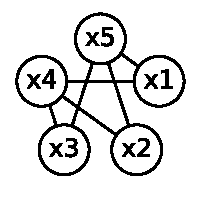
\includegraphics[width=0.25\linewidth]{img/f372738d3845db182fe0b4a3eced9bc2ac778c82a1804f5788cce6bb74ea1beb.pdf}
	\captionof{figure}{Contoh Graf}
	\label{fig:algorithm-example}
\end{minipage}

\vspace{0.5em}

Contoh \foreign{resolving set} berkardinalitas 3 untuk graf ini adalah \(\{v_1, v_2, v_4\}\). Kemudian, karena ia tidak memiliki \foreign{resolving set} berkardinalitas 2, maka kardinalitas minimum \foreign{resolving set}-nya adalah 3. Sehingga, disimpulkan dimensi metriknya adalah 3.

\subsection{\foreign{Brute-force}}
\label{subsec:bf}

Cara paling sederhana untuk menunjukkan bahwa \(k\) adalah kandidat dimensi matrik yang valid adalah dengan mencoba satu per satu himpunan \(W \subseteq V\) berkardinalitas \(k\) hingga ditemukan satu saja \(W\) yang merupakan \foreign{resolving set}. Sebaliknya, untuk menunjukkan bahwa tidak ada \foreign{resolving set} berkardinalitas \(k\), maka harus dicoba habis seluruh kemungkinan himpunan \(W \subseteq V\) berkardinalitas \(k\). Kemudian, untuk menguji apakah \(W\) adalah \foreign{resolving set}, cukup ditunjukkan untuk seluruh kolom di \(P\) bahwa tidak ada \(W\) merupakan himpunan bagian tak sejati dari \(V[P_{*j}]\). Secara terbalik, jika ada saja satu kolom di \(P\) yang menyebabkan \(W \subseteq V[P_{*j}]\), maka \(W\) bukanlah \foreign{resolving set}.

Karena \(P\) berbentuk matriks boolean, akan lebih mudah untuk bekerja dengan representasi \(W\) dalam bentuk boolean juga. Hal ini dapat dilakukan dengan mengkonstruksi vektor boolean \(X \in \Bbb^{|V|}\) yang memiliki sebanyak \(k\) nilai \(\True\). Oleh karena itu, jelas \(W = V[X]\) adalah himpunan berkardinalitas \(k\). Selanjutnya, pengujian apakah \(W\) merupakan himpunan bagian tak sejati dari \(V[P_{*j}]\) dapat dicapai melalui operasi \((X|P_{*j})\). Secara eksplisit:
\vspace{0.25\baselineskip}
\[
	\begin{array}{rl}
		(X|P_{*j}) = P_{*j}  &\iff V[X] \subseteq V[P_{*j}] \\
		(X|P_{*j}) \neq P_{*j}  &\iff V[X] \not\subseteq V[P_{*j}]
	\end{array}
\] \vspace{-1.25\baselineskip} \\

Amatilah, untuk menyatakan bahwa tidak ada \foreign{resolving set} berkardinalitas \(k\), harus diuji habis sebanyak \(\binom{|V|}{k}\) kasus. Sedangkan, secara umum, untuk menemukan satu contoh \foreign{resolving set} berkardinalitas \(k\), akan dibutuhkan banyaknya kasus yang perlu diuji kurang dari \(\binom{|V|}{k}\). Maka dari itu, menemukan satu contoh \foreign{resolving set} berkardinalitas \(k\) "lebih murah" dibandingkan menunjukkan tidak ada \foreign{resolving set} berkardinalitas \(k\). Sehingga, desain algoritma yang melakukan pencarian dari bawah, yaitu secara iteratif menaikkan nilai \(k\) hingga menemukan \foreign{resolving set} pertama dan mengambil kardinalitasnya sebagai dimensi metrik, akan "lebih lambat" dibandingkan desain algoritma yang melakukan pencarian dari atas, yaitu secara iteratif menurunkan nilai \(k\) hingga menemukan kardinalitas pertama yang tidak ada \foreign{resolving set}-nya dan mengambil \(k + 1\) sebagai dimensi metrik.

Dengan demikian, diperolehlah formulasi algoritma penentuan dimensi metrik dan dimensi metrik sisi menggunakan pendekatan \foreign{brute-force} sebagaimana tertera pada \autoref{alg:brute-force}.

\begin{example}
	Ambil graf \autoref{fig:algorithm-example}, dan cari dimensi metriknya menggunakan \autoref{alg:brute-force}.
	\begin{enumerate}
		\item Untuk \(k = 5\), ditemukan \(X = (\True, \True, \True, \True, \True)\) sehingga \(W = \{v_1, v_2,\\ v_3, v_4, v_5\}\) adalah \foreign{resolving set}.
		\item Untuk \(k = 4\), ditemukan \(X = (\True, \True, \True, \True, \False)\) sehingga \(W = \{v_1, v_2,\\ v_3, v_4\}\) adalah \foreign{resolving set}.
		\item Untuk \(k = 3\), ditemukan \(X = (\True, \True, \False, \True, \False)\) sehingga \(W = \{v_1, v_2,\\ v_4\}\) adalah \foreign{resolving set}.
		\item Untuk \(k = 2\), secara habis tidak ada \foreign{resolving set} berkardinalitas 2.
	\end{enumerate}
	Disimpulkan bahwa \(2 + 1 = 3\) adalah dimensi metrik dari graf tersebut.
\end{example}

\subsection{\foreign{Boolean Satisfiability}}
\label{subsec:bs}

Pertama-tama, didefinisikan pemetaan injektif \(\boolmap\) dari \(V\) ke variabel boolean di SMT. Catat bahwa variabel boolean di sini bukanlah elemen di \(\Bbb\), melainkan merupakan variabel abstrak di SMT yang nilainya belum ditentukan. Hanya setelah menjalankan \foreign{solver} barulah dihasilkan \foreign{model} yang elemennya di \(\Bbb\). Dengan demikian, variabel-variabel tersebut digunakan untuk mengkonstruksi \foreign{constraint} sehingga \foreign{model} \(\in \Bbb^{|V|}\) menunjukkan \(W \subseteq V\) yang elemen-elemennya berkoresponden dengan elemen di \(V\) yang \(\boolmap(v_i)\)-nya bernilai \(\True\).

Meskipun secara konsep \(\boolmap(v_i)\) adalah variabel abstrak, secara matematis, tidak dibedakan makna \(\boolmap(v_i)\) antara sebelum dan setelah adanya \foreign{model}. Oleh karena itu, secara praktis, tidak ada salahnya menganggap \(\boolmap(v_i) \in \Bbb\). Cukup dibedakan pemaknaan penggunaan ketika dalam konteks \foreign{constraint}. Menggunakan konvensi ini, \(\boolmap(V) = X\) dapat digunakan langsung untuk \foreign{indexing} pada \(V\), sehingga \(W = V[X] \subseteq V\) terdefinisi dengan baik. Sebelum ada \foreign{model}, \(W\) adalah koresponden dari ruang solusi terhadap \foreign{constraint}, dan setelah ada \foreign{model}, solusi \(W\) adalah himpunan nyata.

\begin{example}
	Bila \(\boolmap(v_i) = x_i\), maka untuk simpul-simpul di \autoref{fig:algorithm-example}, didapatkan \(\boolmap(V) = \{x_1, x_2, x_3, x_4, x_5\} = X\). Kemudian, model \(x_3 = x_4 = x_5 = \True, x_1 = x_2 = \False\), menunjukkan koresponden himpunan \(W = \{x_3, x_4, x_5\} \subseteq V\). Dapat digunakan notasi alternatif \(X = (\False, \False, \True, \True, \True)\) menunjukkan model dan \(W = V[X]\) sebagai koresponden himpunannya.
\end{example}

\begin{algorithm}[H]
	\foreign{Input}:
	\begin{enumerate}
		\item Representasi graf dalam representasi matriks ketetanggaan \(M\).
		\item Mencari dimensi metrik atau dimensi metrik sisi?
	\end{enumerate}
	Prosedur:
	\begin{enumerate}
		\item Hitung \(D^{(V)}\) dari \(M\) menggunakan \foreign{Floyd-Warshall}.
		\item Hitung \(D^{(E)}\) dari \(D^{(V)}\).
		\item Isi \(D\) dengan \(D^{(V)}\) jika mencari dimensi metrik, atau isi \(D\) dengan \(D^{(E)}\) jika mencari dimensi metrik sisi.
		\item Hitung \(B\) dari \(D\).
		\item Hitung \(P\) dari \(B\).
		\item Digunakan variabel \(n\) sebagai banyaknya kolom di \(P\), yaitu \(n :=\) banyak kolom \(P\).
		\item Mulai variabel \(k\) dari banyaknya simpul, yaitu \(k := |V|\).
		\item Selama \(k \geq 0\):
			\begin{enumerate}
				\item Coba satu per satu untuk semua kemungkinan \(X \in \Bbb^{|V|}\) yang memiliki sebanyak \(k\) nilai \(\True\):
					\begin{enumerate}
						\item Mulai variabel \(j\) dari nilai 1, yaitu \(j := 1\).
						\item Selama \(j \leq n\):
							\begin{enumerate}
								\item Jika \((X|P_{*j}) = P_{*j}\), lompat ke tahap (8a).
								\item Tambah \(j\) sebanyak satu, yaitu \(j := j + 1\).
							\end{enumerate}
						\item Lompat ke tahap (8c).
					\end{enumerate}
				\item Lonpat ke tahap (10).
				\item Kurangi \(k\) sebanyak satu, yaitu \(k := k - 1\).
			\end{enumerate}
		\item Simpulkan bahwa 0 adalah dimensi metrik atau dimensi metrik sisi, dan \texttt{BERHENTI}.
		\item Simpulkan bahwa \(k + 1\) adalah dimensi metrik atau dimensi metrik sisi.
	\end{enumerate}
	\caption{\foreign{Brute-force}}
	\label{alg:brute-force}
\end{algorithm}

Kedua, untuk sembarang \(W \subseteq V\), dapat dikonstruksi \foreign{constraint} sedemikian rupa \foreign{model}-nya berkoresponden satu-satu dengan \(W\). Secara umum, variabel yang tidak memiliki restriksi akan memiliki nilai \(\indeterminate\) pada \foreign{model}-nya. Maksud dari \(\indeterminate\) adalah variabel yang bebas; yaitu, tidak peduli apa pun nilai yang ia miliki, kebenaran dari \foreign{constraint} yang ada tidak terpengaruhi oleh variabel tersebut. Ketika \foreign{solver} menghasilkan sebuah \foreign{model}, seluruh variabelnya yang \(\indeterminate\) akan diberi sembarang nilai. Artinya, untuk variabel boolean, ia akan mendapatkan sembarang nilai \(\True\) atau \(\False\). Maka dari itu, agar koresponden \foreign{model}-nya satu-satu dengan himpunan yang dituju, tidak boleh ada variabel yang tidak terestriksi secara tidak sengaja dalam \foreign{constraint} yang dikonstruksikan. Untuk kasus di sini yang memilih tepat \(W\), \foreign{constraint} yang menyatakan pemilihan ini adalah sebagai berikut:

\[
	\combine{\left(}
			{\bigwedge \limits_{\displaystyle v \in W} \boolmap(v)}
	{\right)}{\wedge}{\left(}
			{\bigwedge \limits_{\displaystyle v \in \widetilde{W}} \neg \boolmap(v)}
	{\right)}
\]

\begin{example}
	Untuk \(V = \{v_1, v_2, v_3, v_4, v_5\}\) dan \(W = \{v_3, v_4, v_5\}\), \foreign{constraint} yang menyebabkan koresponden satu-satu antara \(W\) dan \(V[X]\) adalah: \(\neg x_1 \wedge \neg x_2 \wedge x_3 \wedge x_4 \wedge x_5\).
\end{example}

Ketiga, untuk sembarang \(W \subseteq V\), dapat dikonstruksi \foreign{constraint} sedemikian rupa \foreign{model}-nya berkoresponden satu-satu dengan \(\Pcal(W)\). Perhatikan pada konstruksi \foreign{constraint} sebelumnya betapa pentingnya konteks \(V\) yang dimaksud relatif terhadap \(W\) karena \foreign{model} yang menyatakan \(W\) tidak hanya didefinisikan oleh \(W\) sendiri, tetapi juga oleh \(\widetilde{W} = V \setminus W\). Dalam konstruksi \foreign{constraint} untuk \(\Pcal(W)\) ini, hubungan tersebut menjadi lebih kritikal. Karena, terbalik dari perspektif \foreign{power set} pada umumnya, dalam bentuk \foreign{constraint}, definisi \foreign{power set} justru dilihat dari elemen-elemennya yang tidak ada di \(W\). Lebih formalnya dinyatakan oleh ekspresi berikut:
\vspace{-0.25\baselineskip}
\[
	\bigwedge \limits_{\displaystyle v \in \widetilde{W}} \neg \boolmap(v)
\]
Dengan kata lain, seluruh kemungkinan \foreign{model} yang memenuhi \foreign{constraint} ini bebas menetapkan keanggotaan elemen-elemen di \(W\), dan hanya yang di \(W\), sehingga menyatakan seluruh kombinasi yang merepresentasikan \(\Pcal(W)\). Dengan demikian, ruang solusi dari \foreign{model} yang memenuhi \foreign{constraint} tersebut ekivalen dengan \(\Pcal(W)\).

\begin{example}
	Untuk \(V = \{v_1, v_2, v_3, v_4, v_5\}\) dan \(W = \{v_3, v_4, v_5\}\), \foreign{constraint} yang menyebabkan koresponden satu-satu antara \(\Pcal(W)\) dan \(V[X]\) adalah: \(\neg x_1 \wedge \neg x_2\). Setiap \foreign{model} yang memenuhi \(\neg x_1 \wedge \neg x_2\) mewakili satu subset dari \(\{v_3, v_4, v_5\}\).
\end{example}

Akhirnya, dapat dibahas konstruksi \foreign{constraint boolean satisfiability} yang menunjukkan \foreign{resolving set}. Ingat kembali, untuk setiap kolom di \(P\), himpunan \(V[P_{*j}]\) serta seluruh himpunan bagiannya bukanlah \foreign{resolving set}. Maka, \(W \subseteq V\) adalah \foreign{resolving set} jika dan hanya jika \(W\) tidak ada di \(\Pcal(V[P_{*j}])\) untuk setiap kolom di \(P\). Secara formal, ini dapat dinyatakan sebagai berikut:
\vspace{-0.25\baselineskip}
\[
	\bigwedge \limits_{\displaystyle P_{*j} \in P} \neg \left( \bigwedge \limits_{\displaystyle v \in \widetilde{V[P_{*j}]}} \neg \boolmap(v) \right)
\]
Dan dapat disederhakan menjadi:
\vspace{0.25\baselineskip}
\begin{equation}
	\bigwedge \limits_{\displaystyle P_{*j} \in P} \enspace \bigvee \limits_{\displaystyle v \in V[\sim\!P_{*j}]} \boolmap(v)
	\label{eq:boolean-satisfiability-natural}
\end{equation}

\begin{example}
	Ambil graf \autoref{fig:algorithm-example}. \foreign{Constraint} yang berkorespondensi dengan \foreign{resolving set}-nya adalah:
		\[
			( x_1 \vee x_2 ) \wedge \ ( x_1 \vee x_3 ) \wedge \ ( x_2 \vee x_3 ) \wedge \ ( x_4 \vee x_5 )
			\vspace{-1.7em}
		\]
	\label{ex:boolean-satisfiability-natural}
\end{example}

Secara teori, \foreign{constraint} \autoref{eq:boolean-satisfiability-natural} sudah berbentuk \foreign{conjunctive normal form} (CNF). Akan tetapi, ketika menunjukkan \(\unsat\) menggunakan SMT, efektivitasnya sangat bergantung pada \foreign{conflict driven learning}, yaitu metode "penalaran" yang digunakan oleh \foreign{solver} untuk melakukan pemangkasan ruang pencarian. Salah satu sifat yang digunakan oleh \foreign{conflict driven learning} adalah bentuk CNF yang terdiri dari suku-suku positif maupun suku-suku negatif. Sedangkan \autoref{eq:boolean-satisfiability-natural} sepenuhnya hanya memuat suku-suku positif. Bentuk yang sudah diperoleh ini dapat ditransformasikan agar juga memuat suku-suku negatif dengan memfaktorkan keluar "pemilihan" sang himpunan kosong, dengan cara berikut:
\vspace{0.25\baselineskip}
\begin{equation}
	\begin{array}{l}
		\displaystyle \bigwedge \limits_{\displaystyle P_{*j} \in P} \enspace \combine{\left(}{\False}{\right)}{\vee}{\left(}{\bigvee \limits_{\displaystyle v \in V[\sim\!P_{*j}]} \boolmap(v)}{\right)} \\ [18pt]
		\displaystyle = \bigwedge \limits_{\displaystyle P_{*j} \in P} \enspace \combine{\left(}{\combine{\left(}{\bigvee \limits_{\displaystyle v \in V[P_{*j}]} \boolmap(v)}{\right)}{\wedge}{\left(}{\neg \bigvee \limits_{\displaystyle v \in V[P_{*j}]} \boolmap(v)}{\right)}}{\right)}{\vee}{\left(}{\bigvee \limits_{\displaystyle v \in V[\sim\!P_{*j}]} \boolmap(v)}{\right)} \\ [18pt]
		\displaystyle = \bigwedge \limits_{\displaystyle P_{*j} \in P} \enspace \combine{\left(}{\combine{\left(}{\bigvee \limits_{\displaystyle v \in V[P_{*j}]} \boolmap(v)}{\right)}{\vee}{\left(}{\bigvee \limits_{\displaystyle v \in V[\sim\!P_{*j}]} \boolmap(v)}{\right)}}{\right)}{\\[18pt]\qquad\qquad\wedge}{\left(}{\combine{\left(}{\neg \bigvee \limits_{\displaystyle v \in V[P_{*j}]} \boolmap(v)}{\right)}{\vee}{\left(}{\bigvee \limits_{\displaystyle v \in V[\sim\!P_{*j}]} \boolmap(v)}{\right)}}{\right)} \\ [18pt]
		\displaystyle = \bigwedge \limits_{\displaystyle P_{*j} \in P} \enspace \combine{\left(}{\bigvee \limits_{\displaystyle v \in V} \boolmap(v)}{\right)}{\wedge}{\left(}{\bigvee \limits_{\displaystyle v \in V[P_{*j}]} \boolmap(v)\ \implies \bigvee \limits_{\displaystyle v \in V[\sim\!P_{*j}]} \boolmap(v)}{\right)} \\ [18pt]
		\displaystyle = \combine{\left(}{\bigvee \limits_{\displaystyle v \in V} \boolmap(v)}{\right)}{\wedge}{\left(}{\bigwedge \limits_{\displaystyle P_{*j} \in P} \enspace \left( \bigvee \limits_{\displaystyle v \in V[P_{*j}]} \boolmap(v)\ \implies \bigvee \limits_{\displaystyle v \in V[\sim\!P_{*j}]} \boolmap(v) \right)}{\right)} \\ [18pt]
	\end{array}
	\label{eq:boolean-satisfiability}
\end{equation}
\vspace{-1.5\baselineskip}

\begin{example}
	Berikut adalah hasil dari pemfaktoran \autoref{ex:boolean-satisfiability-natural}.
	\[
		\smash[b]{
		\begin{array}{c}
			x_1 \vee x_2 \vee x_3 \vee x_4 \vee x_5 \\ [4pt]
			x_3 \vee x_4 \vee x_5 \implies x_1 \vee x_2 \\
			x_2 \vee x_4 \vee x_5 \implies x_1 \vee x_3 \\
			x_1 \vee x_4 \vee x_5 \implies x_2 \vee x_3 \\
			x_1 \vee x_2 \vee x_3 \implies x_4 \vee x_5
		\end{array}
		} \vspace{.5em}
	\]
	\label{ex:boolean-satisfiability}
\end{example}
\vspace{0.25\baselineskip}

Karena ruang solusi \foreign{model} yang memenuhi \foreign{constraint} tersebut sudah menunjukkan \foreign{resolving set}, maka algoritma yang perlu dirancang cukup mencari \foreign{resolving set} dengan kardinalitas terendah dari ruang solusi. Ini dapat dilakukan dengan mudah menggunakan \foreign{constraint} \(\AtLeast\) dan \(\AtMost\) yang memaksa banyaknya variabel boolean bernilai \(\True\) secara berturut-turut kurang dari atau sama dengan dan lebih dari atau sama dengan \(k\).

Secara historis, SMT paling efektif ketika bekerja langsung dengan bentuk CNF. Akan tetapi, SMT \foreign{modern} sudah tidak lagi terbatasi oleh \foreign{implementation detail} seperti ini, sebagaimana yang telah dibahasa pada Pendahuluan. Maka dari itu, \foreign{solver} sekarang sudah memiliki \foreign{higher level construct} dan justru lebih banyak diuntungkan ketika bekerja langsung dalam bentuk tersebut. \foreign{Constraint} \(\AtLeast\) dan \(\AtMost\) merupakan salah satu contoh dari \foreign{higher level construct} yang ada dalam SMT. Namun, tidak ada salahnya untuk memahami bagaimana bentuk-bentuk ini dapat direpresentasikan menggunakan operasi konjungsi dan disjungsi yang lebih sederhana. Berikut adalah salah satu \foreign{encoding} yang mungkin dilakukan untuk menyatakan kedua \foreign{constraint} tersebut. Catat, notasi \(\displaystyle \binom{V}{n} = \{W \subseteq V : |V| = n\}\) menunjukkan himpunan yang memuat seluruh himpunan bagian \(V\) dengan kardinalitas \(n\).
\[
	\AtLeast(V, n) = \displaystyle \bigvee \limits_{\displaystyle W \in \binom{V}{n}} \enspace \bigwedge \limits_{\displaystyle v \in W} \boolmap(v)
\]

\[
	\AtMost(V, n) = \displaystyle \bigvee \limits_{\displaystyle W \in \binom{V}{n}} \enspace \bigwedge \limits_{\displaystyle v \in \widetilde{W}} \neg \boolmap(v)
\]

Secara umum, menunjukkan \(\sat\) dalam SMT lebih murah dari pada menunjukkan \(\unsat\). Hal ini karena secara fundamental, SMT adalah proses mencari \foreign{model}. Oleh karena itu, untuk menunjukkan \(\sat\), cukup dicari satu saja contoh yang memenuhi \foreign{constraint}. Sedangkan untuk menunjukkan \(\unsat\), harus secara habis dibuktikan bahwa tidak ada satu pun \foreign{model} yang dapat memenuhi \foreign{constraint}.

Dengan demikian, didapatkan desain \autoref{alg:boolean-satisfiability} yang melakukan pencarian dari atas. Digunakan \(\AtLeast\) dan \(\AtMost\) secara bersamaan untuk memaksa mencari \foreign{model} berkardinalitas tepat sama dengan \(k\). Dimulai dari nilai \(k\) tertinggi, lalu secara iteratif menurunkan nilai \(k\) hingga menemukan kardinalitas pertama yang menyebabkan \(\unsat\), dan mengambil \(k + 1\) sebagai dimensi metrik.

\begin{example}
	Ambil graf \autoref{fig:algorithm-example}, dan cari dimensi metriknya menggunakan \autoref{alg:boolean-satisfiability}. \foreign{Constraint} yang digunakan sesuai dengan \autoref{ex:boolean-satisfiability}. Kemudian, untuk masing-masing tahap berikut, diterapkan \foreign{constraint} tambahan \(\AtLeast\) dan \(\AtMost\) sama dengan \(k\).
	\begin{enumerate}
		\item Untuk \(k = 5\), ditemukan \(\sat\).
		\item Untuk \(k = 4\), ditemukan \(\sat\).
		\item Untuk \(k = 3\), ditemukan \(\sat\).
		\item Untuk \(k = 2\), ditemukan \(\unsat\).
	\end{enumerate}
	Disimpulkan bahwa \(2 + 1 = 3\) adalah dimensi metrik dari graf tersebut.
\end{example}

\subsection{\foreign{Linear Integer Arithmetic}}

Seperti pemetaan injektif \(\boolmap\), di sini didefinisikan pemetaan injektif \(\intmap\) dari \(V\) ke variabel \foreign{integer} di SMT. Dengan membatasi \(0 \leq \intmap(v_i) \leq 1\), seperti halnya koresponden keanggotaan simpul dalam \(W\) bergantung dari nilai \(\True\) untuk \(\boolmap(v_i)\), nilai \(1\) untuk \(\intmap(v_i)\) menunjukkan korespondensi keanggotaan dan nilai \(0\) untuk tidak. Sehingga, pemetaan \foreign{resolving set} ke dalam \foreign{constraint boolean satisfiability} dapat diangkat secara langsung ke bentuk \foreign{linear integer arithmetic} dengan melakukan translasi berikut:
\vspace{0.2\baselineskip}
\[
	\bigvee \limits_{\displaystyle v \in W} \boolmap(v)
	\iff
	\sum \limits_{\displaystyle v \in W} \intmap(v) \enspace \geq 1
\]

\begin{algorithm}[H]
	\foreign{Input}:
	\begin{enumerate}
		\item Representasi graf dalam representasi matriks ketetanggaan \(M\).
		\item Mencari dimensi metrik atau dimensi metrik sisi?
	\end{enumerate}
	Prosedur:
	\begin{enumerate}
		\item[1--5.] Sama seperti pada \autoref{alg:brute-force}.
		\setcounter{enumi}{5}
		\item Tambahkan \foreign{constraint} berdasarkan \autoref{eq:boolean-satisfiability} dari \(P\) ke \foreign{solver} SMT.
		\item Mulai variabel \(k\) dari banyaknya simpul, yaitu \(k := |V|\).
		\item Selama \(k \geq 0\):
			\begin{enumerate}
					\item Tambahkan \foreign{constraint} \(\AtLeast\) dan \(\AtMost\) sama dengan \(k\).
					\item Jalankan \foreign{solver} untuk mencari \foreign{model}.
					\item Jika dihasilkan \(\unsat\), lompat ke tahap (10).
					\item Hapus \foreign{constraint} \(\AtLeast\) dan \(\AtMost\) yang ditambahkan sebelumnya.
					\item Kurangi \(k\) sebanyak satu, yaitu \(k := k - 1\).
			\end{enumerate}
		\item Simpulkan bahwa 0 adalah dimensi metrik atau dimensi metrik sisi, dan \texttt{BERHENTI}.
		\item Simpulkan bahwa \(k + 1\) adalah dimensi metrik atau dimensi metrik sisi.
	\end{enumerate}
	\caption{\foreign{Boolean Satisfiability}}
	\label{alg:boolean-satisfiability}
\end{algorithm}
\vspace{-\baselineskip}

\noindent Dan didapat bentuk dari \autoref{eq:boolean-satisfiability-natural} dalam \foreign{linear integer arithmetic} sebagai berikut:
\vspace{-0.5\baselineskip} \\
\begin{equation}
	\bigwedge \limits_{\displaystyle P_{*j} \in P} \enspace \sum \limits_{\displaystyle v \in V[\sim\!P_{*j}]} \intmap(v) \enspace \geq 1
	\label{eq:linear-integer-arithmetic-natural}
\end{equation}

\vspace{-0.5\baselineskip}
\begin{example}
	Ambil graf \autoref{fig:algorithm-example}. Misalnya \(\intmap(v_i) = x_i\), maka \foreign{constraint} yang berkorespondensi dengan \foreign{resolving set}-nya dalam \foreign{linear integer arithmetic} adalah:
	\vspace{0.2\baselineskip}
	\[
		\smash[b]{
		\begin{array}{c}
			x_1 + x_2 \geq 1 \\
			x_1 + x_3 \geq 1 \\
			x_2 + x_3 \geq 1 \\
			x_4 + x_5 \geq 1 \\ [8pt]
			0 \leq x_1 \leq 1,\enspace
			0 \leq x_2 \leq 1,\enspace
			0 \leq x_3 \leq 1,\enspace
			0 \leq x_4 \leq 1,\enspace
			0 \leq x_5 \leq 1
		\end{array}
		} \vspace{1em}
	\]
\end{example}

Selanjutnya, untuk \foreign{constraint} \(\AtLeast\) dan \(\AtMost\), dapat dinyatakan dalam \foreign{linear integer arithmetic} dengan lebih sederhana sebagai:
\vspace{0.25\baselineskip}
\begin{equation}
	\sum \limits_{\displaystyle v \in V} \intmap(v) \enspace = k
	\label{eq:linear-integer-arithmetic-cardinality}
\end{equation}

Perhatikan bentuk jumlahan ini yang lebih ekspresif dari pada \(\AtLeast\) dan \(\AtMost\). Menggunakan persamaan ini, \autoref{eq:linear-integer-arithmetic-natural} dapat ditransformasi menjadi relatif terhadap kardinalitas \(k\) seperti berikut:
\begin{equation}
	\bigwedge \limits_{\displaystyle P_{*j} \in P} \enspace \sum \limits_{\displaystyle v \in V[P_{*j}]} \intmap(v) \enspace \leq k - 1
	\label{eq:linear-integer-arithmetic}
\end{equation}

Sama seperti transformasi \autoref{eq:boolean-satisfiability-natural} ke \autoref{eq:boolean-satisfiability} yang membantu \foreign{conflict driven learning}, transformasi di \foreign{linear integer arithmetic} dari \autoref{eq:linear-integer-arithmetic-natural} ke \autoref{eq:linear-integer-arithmetic} juga membantu SMT dalam pemangkasan ruang pencarian.

\begin{example}
	Untuk graf \autoref{fig:algorithm-example}, \foreign{constraint} yang berkorespondensi dengan \foreign{resolving set} berkardinalitas \(k\) adalah:
	\[
		\smash[b]{
		\begin{array}{c}
			x_1 + x_2 + x_3 + x_4 + x_5 = k \\ [8pt]
			x_3 + x_4 + x_5 \leq k - 1 \\
			x_2 + x_4 + x_5 \leq k - 1 \\
			x_1 + x_4 + x_5 \leq k - 1 \\
			x_1 + x_2 + x_3 \leq k - 1 \\ [8pt]
			0 \leq x_1 \leq 1,\enspace
			0 \leq x_2 \leq 1,\enspace
			0 \leq x_3 \leq 1,\enspace
			0 \leq x_4 \leq 1,\enspace
			0 \leq x_5 \leq 1
		\end{array}
		} \vspace{1.5em}
	\]
	\label{ex:linear-integer-arithmetic-constraint}
\end{example}
\vspace{0.5\baselineskip}

Dengan demikian, didapatkan desain algoritma yang menggunakan \foreign{linear integer arithmetic}.

\begin{example}
	Ambil graf \autoref{fig:algorithm-example}, dan cari dimensi metriknya menggunakan \autoref{alg:linear-integer-arithmetic}. Setelah menetapkan \foreign{constraint} \(0 \leq x_i \leq 1\) untuk setiap variabel \foreign{integer}-nya, \foreign{constraint} yang digunakan pada setiap tahapannya bersesuaian dengan yang telah tertera pada \autoref{ex:linear-integer-arithmetic-constraint}.
	\begin{enumerate}
		\item Untuk \(k = 5\), ditemukan \(\sat\).
		\item Untuk \(k = 4\), ditemukan \(\sat\).
		\item Untuk \(k = 3\), ditemukan \(\sat\).
		\item Untuk \(k = 2\), ditemukan \(\unsat\).
	\end{enumerate}
	Disimpulkan bahwa \(2 + 1 = 3\) adalah dimensi metrik dari graf tersebut.
\end{example}

\subsection{\foreign{Pseudo Boolean}}

Pada akhirnya, sampailah di penghujung desain algoritma dimensi metrik menggunakan SMT. Cermati bentuk \foreign{constraint} yang terdapat dalam \foreign{linear integer arithmetic} sudah sesuai dengan representasi \foreign{constraint} yang dibutuhkan dalam \foreign{pseudo boolean}. Maka dari itu, konstruksi \foreign{constraint} dapat diturunkan kembali menggunakan variabel boolean dari pada \foreign{integer}, tetapi menggunakan teori yang lebih tinggi dari \foreign{boolean satisfiability}, yaitu \foreign{pseudo boolean}. Di sini, didapatkan kembali representasi natural keanggotaan sebagai nilai \(\True\), dan secara bersamaan dapat diekspresikan bentuk \foreign{constraint} yang memuat logika kardinalitas secara lebih natural. Dengan demikian, \autoref{eq:linear-integer-arithmetic-cardinality} dan \autoref{eq:linear-integer-arithmetic} dapat translasikan langsung menjadi pseudo boolean sebagai berikut:

\begin{equation}
	\sum \limits_{\displaystyle v \in V} \boolmap(v) \enspace = k
	\label{eq:pseudo-boolean-cardinality}
\end{equation}

\begin{equation}
	\bigwedge \limits_{\displaystyle P_{*j} \in P} \enspace \sum \limits_{\displaystyle v \in V[P_{*j}]} \boolmap(v) \enspace \leq k - 1
	\label{eq:pseudo-boolean}
\end{equation}

Meskipun perubahan yang dilakukan hanyalah membawa turun dari \foreign{linear integer arithmetic} ke \foreign{pseudo boolean}, dengan bentuk \foreign{constraint} yang kurang lebih sama persis, ketika tidak ada \foreign{expresiveness} yang hilang, maka secara umum \foreign{solver} yang menggunakan \foreign{pseudo boolean} akan lebih efektif dibandingkan yang menggunakan \foreign{linear integer arithmetic}.

\begin{algorithm}[H]
	\foreign{Input}:
	\begin{enumerate}
		\item Representasi graf dalam representasi matriks ketetanggaan \(M\).
		\item Mencari dimensi metrik atau dimensi metrik sisi?
	\end{enumerate}
	Prosedur:
	\begin{enumerate}
		\item[1--5.] Sama seperti pada \autoref{alg:boolean-satisfiability}.
		\setcounter{enumi}{5}
		\item Tambahkan \foreign{constraint} \(0 \leq \intmap(v_i) \leq 1\) untuk semua \(v_i \in V\) ke \foreign{solver} SMT.
		\item Mulai variabel \(k\) dari banyaknya simpul, yaitu \(k := |V|\).
		\item Selama \(k \geq 0\):
			\begin{enumerate}
					\item Tambahkan \foreign{constraint} berdasarkan \autoref{eq:linear-integer-arithmetic-cardinality}, dan berdasarkan \autoref{eq:linear-integer-arithmetic} dari \(P\), ke \foreign{solver} SMT.
					\item Jalankan \foreign{solver} untuk mencari \foreign{model}.
					\item Jika dihasilkan \(\unsat\), lompat ke tahap (10).
					\item Hapus \foreign{constraint} yang ditambahkan dari tahap (8a) sebelumnya.
					\item Kurangi \(k\) sebanyak satu, yaitu \(k := k - 1\).
			\end{enumerate}
		\item Simpulkan bahwa 0 adalah dimensi metrik atau dimensi metrik sisi, dan \texttt{BERHENTI}.
		\item Simpulkan bahwa \(k + 1\) adalah dimensi metrik atau dimensi metrik sisi.
	\end{enumerate}
	\caption{\foreign{Linear Integer Arithmetic}}
	\label{alg:linear-integer-arithmetic}
\end{algorithm}

\begin{example}
	Ambil graf \autoref{fig:algorithm-example}. Jika \(\boolmap(v_i) = x_i\), maka \foreign{constraint} yang berkorespondensi dengan \foreign{resolving set} berkardinalitas \(k\) adalah:
	\[
		\smash[b]{
		\begin{array}{c}
			x_1 + x_2 + x_3 + x_4 + x_5 = k \\ [8pt]
			x_3 + x_4 + x_5 \leq k - 1 \\
			x_2 + x_4 + x_5 \leq k - 1 \\
			x_1 + x_4 + x_5 \leq k - 1 \\
			x_1 + x_2 + x_3 \leq k - 1
		\end{array}
		} \vspace{.6em}
	\]
	\label{ex:pseudo-boolean-constraint}
\end{example}

Sehingga, didapat desain algoritma yang menggunakan \foreign{pseudo boolean}.

\begin{example}
	Untuk graf \autoref{fig:algorithm-example}, mencari dimensi metriknya menggunakan \autoref{alg:pseudo-boolean}, dapat dilakukan dengan mengambil pada setiap tahapannya \foreign{constraint} yang telah tertera pada \autoref{ex:pseudo-boolean-constraint}.
	\begin{enumerate}
		\item Untuk \(k = 5\), ditemukan \(\sat\).
		\item Untuk \(k = 4\), ditemukan \(\sat\).
		\item Untuk \(k = 3\), ditemukan \(\sat\).
		\item Untuk \(k = 2\), ditemukan \(\unsat\).
	\end{enumerate}
	Disimpulkan bahwa \(2 + 1 = 3\) adalah dimensi metrik dari graf tersebut.
\end{example}

\begin{algorithm}[H]
	\foreign{Input}:
	\begin{enumerate}
		\item Representasi graf dalam representasi matriks ketetanggaan \(M\).
		\item Mencari dimensi metrik atau dimensi metrik sisi?
	\end{enumerate}
	Prosedur:
	\begin{enumerate}
		\item[1--5.] Sama seperti pada \autoref{alg:linear-integer-arithmetic}.
		\setcounter{enumi}{5}
		\item Mulai variabel \(k\) dari banyaknya simpul, yaitu \(k := |V|\).
		\item Selama \(k \geq 0\):
			\begin{enumerate}
					\item Tambahkan \foreign{constraint} berdasarkan \autoref{eq:pseudo-boolean-cardinality}, dan berdasarkan \autoref{eq:pseudo-boolean} dari \(P\), ke \foreign{solver} SMT.
					\item Jalankan \foreign{solver} untuk mencari \foreign{model}.
					\item Jika dihasilkan \(\unsat\), lompat ke tahap (9).
					\item Hapus \foreign{constraint} yang ditambahkan dari tahap (7a) sebelumnya.
					\item Kurangi \(k\) sebanyak satu, yaitu \(k := k - 1\).
			\end{enumerate}
		\item Simpulkan bahwa 0 adalah dimensi metrik atau dimensi metrik sisi, dan \texttt{BERHENTI}.
		\item Simpulkan bahwa \(k + 1\) adalah dimensi metrik atau dimensi metrik sisi.
	\end{enumerate}
	\caption{\foreign{Pseudo Boolean}}
	\label{alg:pseudo-boolean}
\end{algorithm}
